
%
% conclusions
%

\chapter{Conclusions \& Outlook}
\label{chapter:conclusions-outlook}

\section{Performance evaluation}
\label{chapter:performance}

Performant real-time clustering is the main objective of this thesis as formulated in chapter \ref{chapter:objective-performance}. As a requirement, the algorithm should cluster in real-time to support dynamic queries and cluster up to 1,000,000 items within less than one second.

The configuration of the demo use case implementation described in chapter \ref{chapter:use-case-demo} was used to do automated performance testing of the different clustering algorithms. A \textit{Bash}\footnote{\url{http://en.wikipedia.org/wiki/Bash\_(Unix\_shell)}} script was created to test the performance of the clustering algorithm based against an incrementing number of items.

\begin{figure}[h]
  \begin{center}
    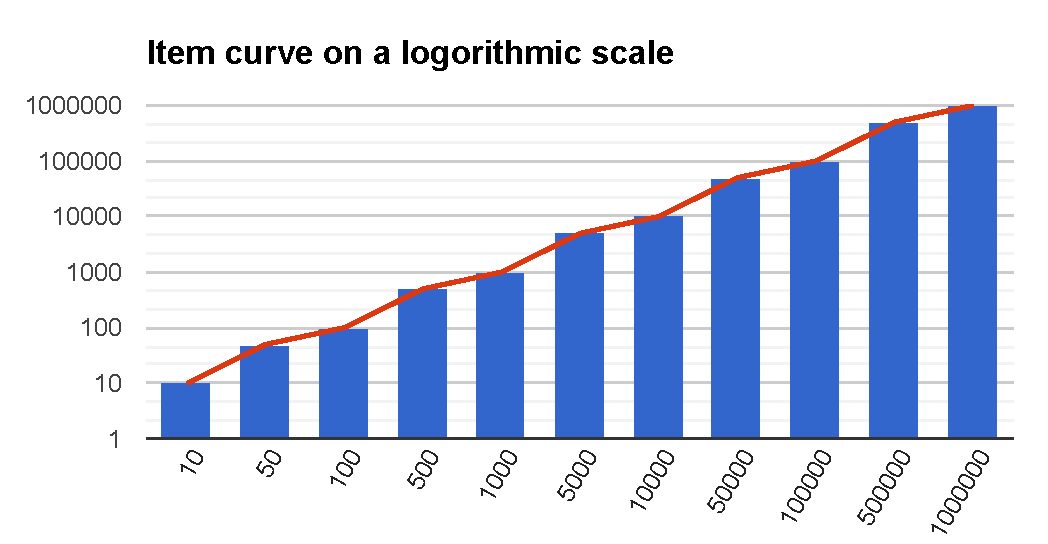
\includegraphics[width=0.8\textwidth]{figures/performance_items.pdf}
    \caption{Item curve on a logorithmic scale.}
    \label{fig:performance-items}
  \end{center}
\end{figure}

The script exponentially increases items to test the clustering performance from a base 10 up to 1,000,000 items. Between every two steps of the exponential function, an intermediary step of the half of the two steps will be inserted. While the exponential mean value for example between 100 and 1000 items would be 316.2, this approach inserts 500 to improve readability of the results for humans. The resulting curve of items tested is visualized in figure \ref{fig:performance-items}.

The \textit{ab} command of the ApacheBench\footnote{\url{http://en.wikipedia.org/wiki/ApacheBench}} is used to sequentially repeat the same requests and calculate a mean response time value. Hereby the script tries to circumvent variations caused by external factors as the server hardware and operating system.

The results of the performance benchmark have been extracted and aggregated into a chart as show in figure \ref{fig:algorithm-performance}. It is clearly shown that that the three implemented algorithms perform very differently. Each algorithm scales up to a certain number of items, while beyond this threshold, performance decreases significantly. The PHP-based clustering algorithm is very limited in such that requests for up to 1,000 clustered items can be completed within one second. The MySQL-based clustering approach scales much better but requests get slow beyond 100,000 items. The most performant algorithm implementation is the Solr-based one that server 1,000,000 items still in a reasonable amount of time. 

\begin{figure}[h]
  \begin{center}
    \hspace*{-1.5cm}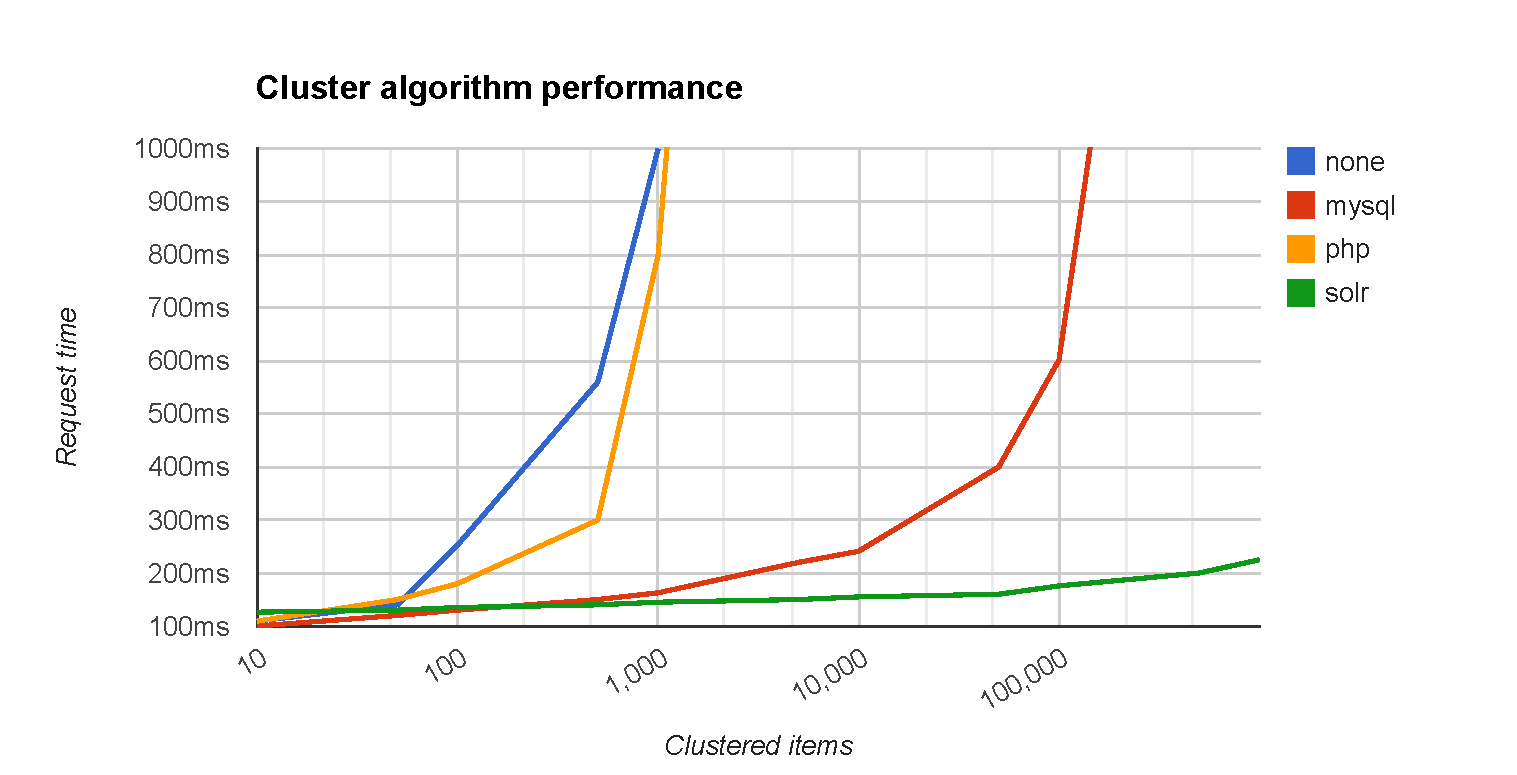
\includegraphics[width=1.3\textwidth]{figures/geocluster_algorithm_performance.pdf}
    \caption{Geocluster performance in milliseconds per algorithm and number of items.}
    \label{fig:algorithm-performance}
  \end{center}
\end{figure}

A deeper analysis of the PHP-based algorithm clearly shows that the most time-consuming part of the algorithm is creating the clusters based on Geohash. As all unclustered items need to processed after executing the database query have to be processed, this part takes the most time. In an example based on a query with 9270 items, the entire roundtrip between client and server takes 26.71 seconds. Querying the items just took 100ms. With 24.32 seconds, the Geohash-based pre-clustering consumes the major part of the execution time. For the same amount of items, a request using the MySQL-based algorithm was completed within 194 ms. In this case, the query was completed after 80 ms and the while clustering process was finished 8 ms seconds later. The remainder of the processing time was consumed by Drupal performing non-clustering related processing before and at the end of the request. This example shows, how shifting the main clustering task into the database can increase performance for a certain range of number of items. As stated before, when approaching 100,000 items the MySQL-based algorithm is getting significantly slower, as the query itself takes longer.

Given the numbers, the performance criterion of this thesis could be fulfilled. While the PHP-based implementation isn't really usable, MySQL-based and Solr-based clustering can be used to create performant, interactive maps with Drupal for item sets up to at least 1,000,000 items. While we know that MySQL-based clustering only scales up to 100,000 items, the threshold for Solr-based clustering wasn't determined as tests were limited up to 1,000,000 items. It is expected that there is room for improvements and optimizations for all of the algorithms.


\textbf{Real-world scenario}. In a second step, the performance of Geocluster has been evaluated based using a more realistic setup. The Drupaljobs test site based on Recruiter, explained in chapter \ref{chapter:use-case-georecruiter}, was used as a test environment. A scenario for performance testing the map was created using the Selenium IDE\footnote{\url{http://docs.seleniumhq.org/projects/ide/}} for the Firefox\footnote{\url{http://www.mozilla.org/en-US/firefox}} web browser. Selenium IDE is an integrated development environment, that allows to record and play back tests. In combination with the Firebug\footnote{\url{http://getfirebug.com/}} browser extension, the response times for the map interaction have been captured and evaluated.

The test scenario opens the website with a map that displays job offers using either the MySQL-based or the Solr-based clustering algorithm. The larger test data set of the Drupaljobs test site with 100,000 items within the U.S. was chosen. As the previous performance test indicates, this amount of items can't be processed efficiently using the PHP-based implementation of the clustering algorithm, this is why PHP-based and Solr-based clustering were evaluated. In comparison to the previous performance test, this test aims at simulating standard user behavior in the browser. Thus, a Selenium script captured a sequence of user interaction on the map as zooming into particular areas of the map. In total, one sequence consists of the zooming into 4 different areas of the map on 5 zoom levels and zooming out again which sums up to 21 request per sequence. As the bounding box strategy of the Javascript mapping automatically applies a filter to the query for the current viewport, a different sub-set of the 100,000 items will get queried per request. The test sequence was repeated 5 times for each of the two clustering algorithm implementations and the results captured using the Firebug Net Panel log.

\begin{figure}[h]
  \begin{center}
  \hspace*{-1.5cm}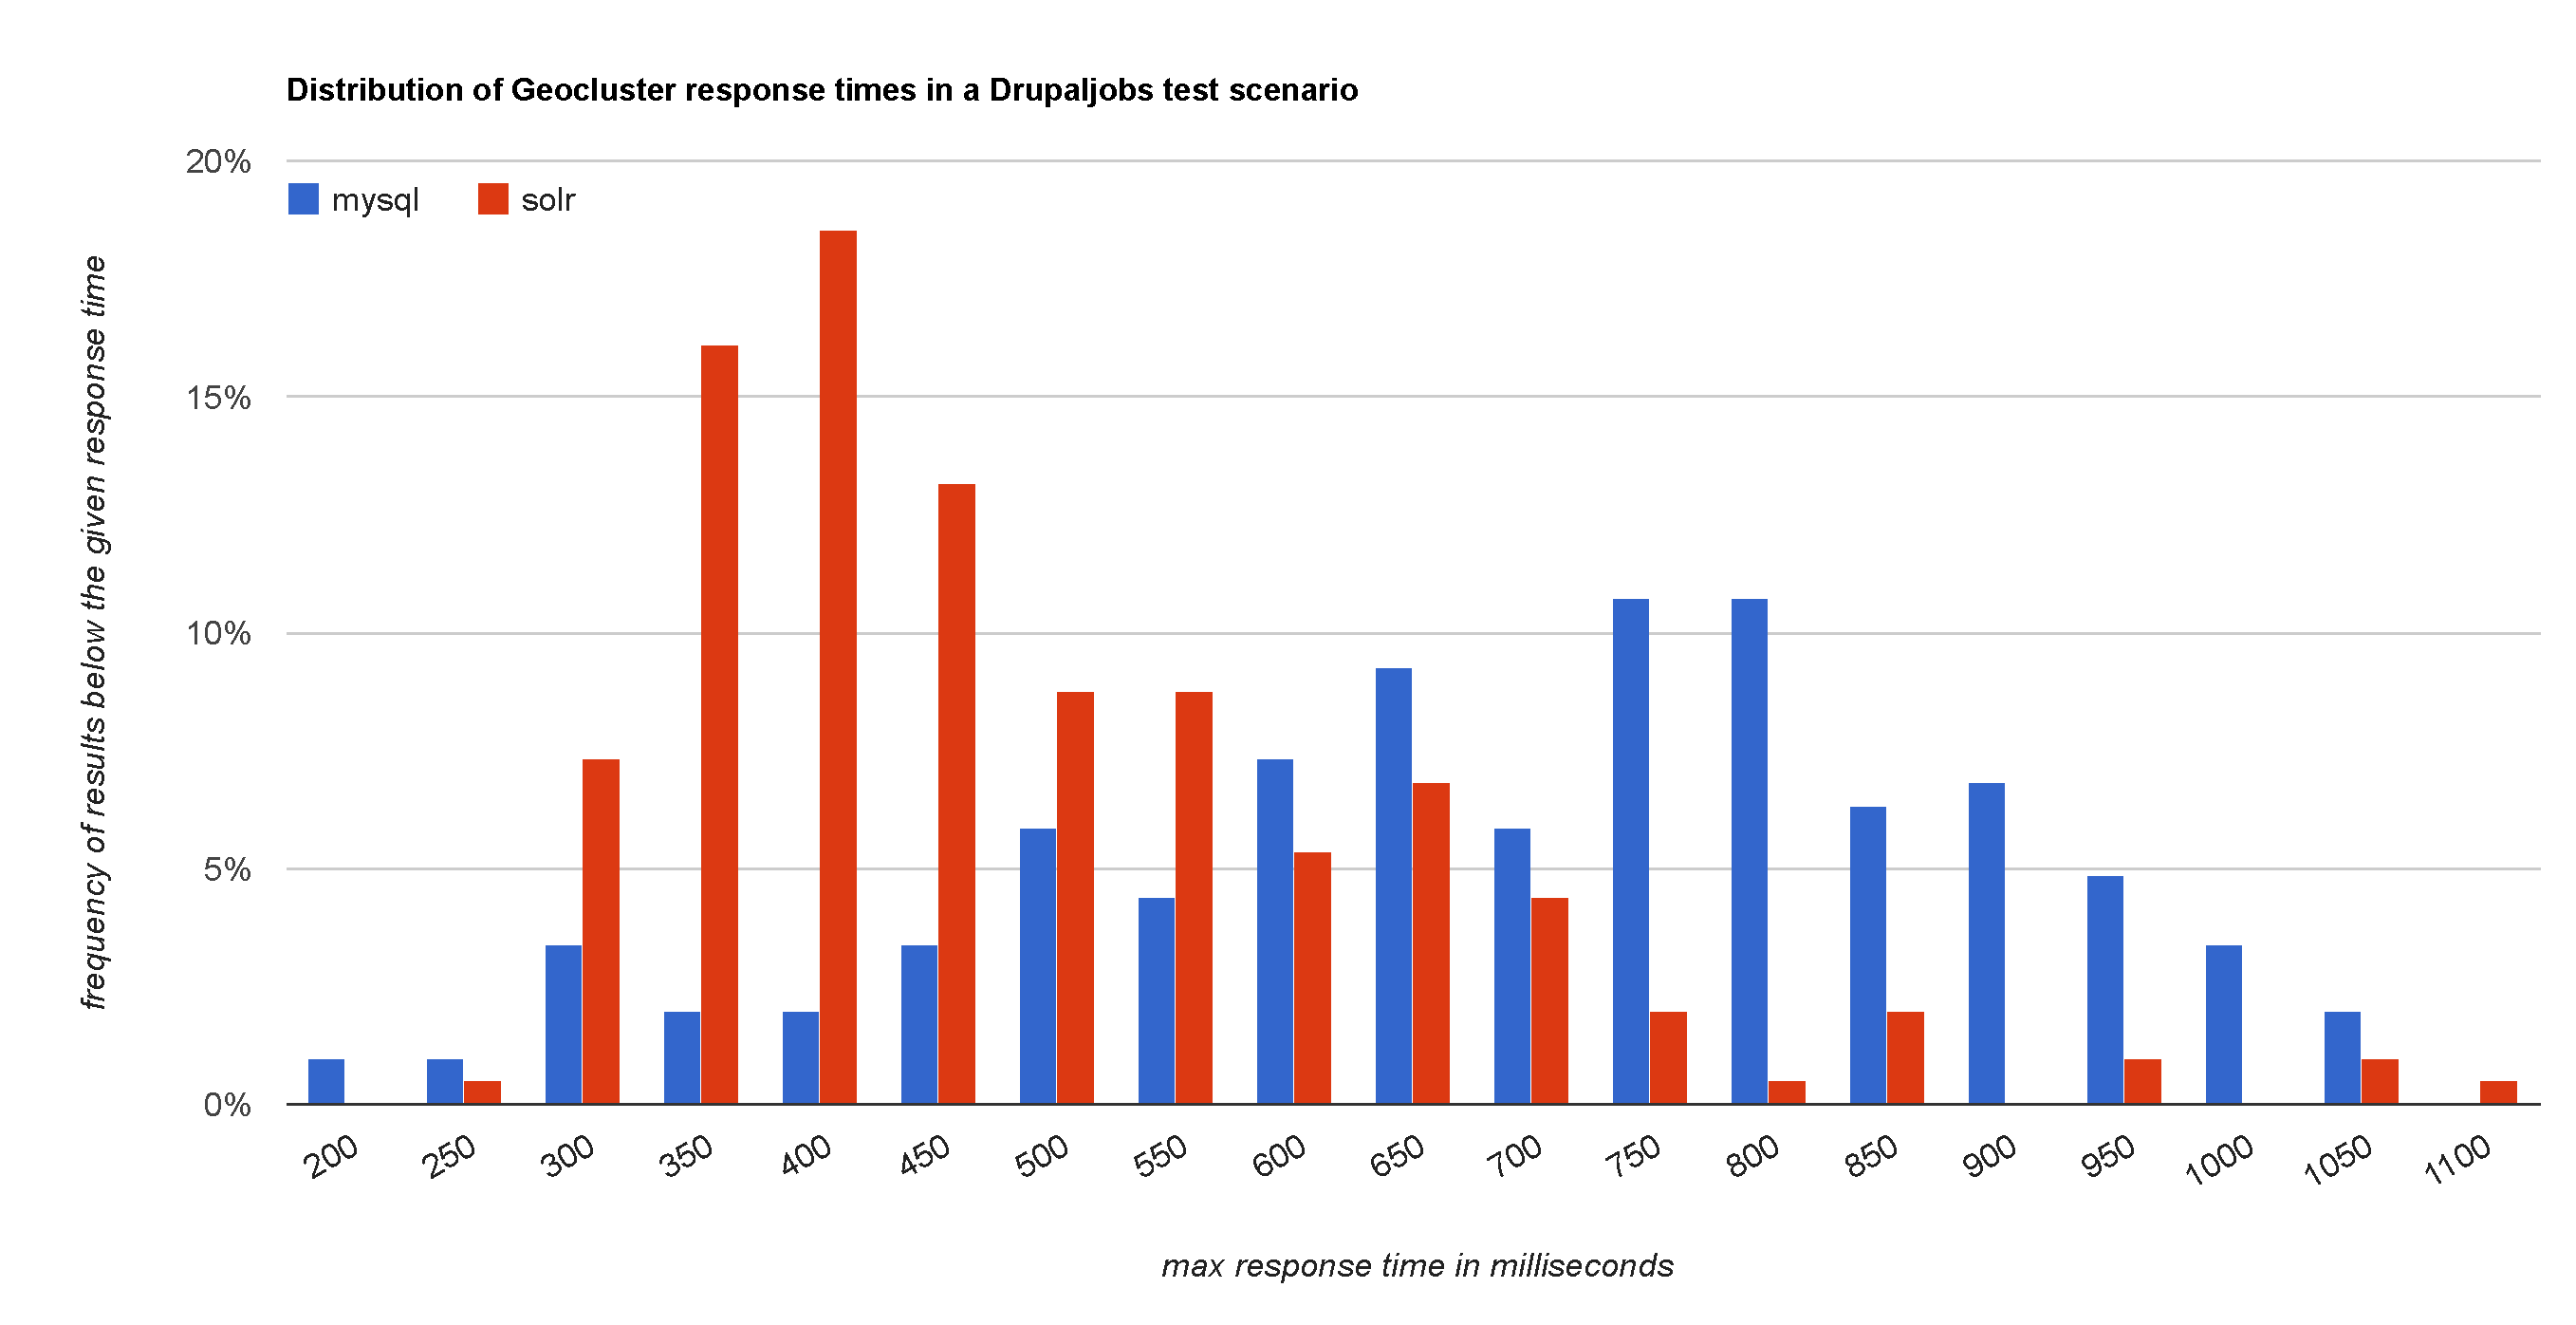
\includegraphics[width=1.2\textwidth]{figures/geocluster_response_time_distribution.pdf}
    \caption{Distribution of Geocluster response times for MySQL- and Solr-based clustering in a Drupaljobs test scenario with 100,000 items.}
    \label{fig:real-performance}
  \end{center}
\end{figure}

The results of the real-world test scenario have been evaluated into a histogram that shows the distribution of response times and which is illustrated in figure \ref{fig:real-performance}. The Solr-based clustering implementation shows a highest frequency of response times under 400 milliseconds, while the response times of the MySQL-based implementation have a highest frequency below 750 and 800 milliseconds. These real-world test results yield slower response times than the previous performance test where Solr-based response times where constantly below 300 ms. This is might be caused by external factors: in the first case, a plain Drupal installation was being used and queried locally from the server, while the second test case was built on top of an existing Drupal site with a larger number of modules installed and queries where done from a local machine, adding network latency.

Another performance-related aspect is cachability of responses and results. Apache Solr and Drupal itself already incorporate various caching layers. Caching clustered results for the server-side clustering solution mainly depends on the parameters of the Bounding Box strategy. As currently, every minor change to the bounding box will issue a different request to the server, these can't be cached efficiently. A possible solution that has been discussed\footnote{\url{http://drupal.org/node/1868982}}, is to define fixed steps for the bounding box in order to produce repeating requests that can be cached. 



\section{Visual evaluation}

The second objective from chapter \ref{chapter:objective-usability} defines the vague goal of supporting the user by compacting the amount of information that is visualized. To do so, two visualizations have been provided: first, the Client-side Geocluster Visualization component as visualized in figure \ref{fig:geocluster-demo-site} of chapter \ref{chapter:geocluster-vis} and second, an alternative visualization similar to the Leaflet.markercluster library for the GeoRecruiter use case, see figure \ref{fig:drupaljobs-geocluster-solr} in chapter \ref{chapter:use-case-georecruiter}.

Both implementations fulfill most of the clutter reduction criteria from chapter \ref{clutter-reduction}:

\begin{enumerate}

\item \textit{Overlap} is avoided by visualizing a non-overlapping clustering of points, as created by geohash-based clustering algorithm of Geocluster.

\item \textit{Spatial information} is expressed as an aggregate of latitude and longitude values for each cluster, approximating its centroid. One problem with the current implementations is, that clusters aren't ``stable''. In some experiments, changes to the bounding box will cause a change of cluster assignment. Intuitively, this leads to confusion of the user and should be investigated upon further. 

\item The Leaflet Bounding Box strategy implementation allows to \textit{localize} the view by panning and zooming and therefore reduce the display to a specific region.

\item \textit{Scalability} is provided by the underlying clustering algorithm, as evaluated in the previous section.

\item The configuration options of Geocluster, presented in chapter \ref{chapter:geocluster-config}, allow to \textit{adjust} the minimum distance between clusters. Additional configuration options are provided by the Views integration of the Geocluster module. Still, the configuration options could be expanded for example to control visual parameters of clusters. 

\item The criterion of \textit{showing point/line attributes} is fulfilled only in a very limited way. Both implementations are currently restricted to displaying the number of items within a cluster as the only aggregate value. In order to support complex visualization techniques for multivariate data as discussed in chapter \ref{chapter:cluster-vis}, the clustering implementation needs to provide the required, aggregate values of the underlying data.

\item As explained in the discussion of the \textit{discriminating points/lines} criterion, its definition seems unclear. Clustered items and individual points are visualized in a different way, which can be seen as a fulfillment. On the other hand, the visualization currently doesn't provide any means of inspecting clusters. Only a list of identifiers of the items within a cluster is provided. Based upon the identifiers, a popup could be used to visualize the items a in more detailed way.

\item With regards to \textit{overlap density}, the number of items within clusters is indicated by both visualizations, but using different means. The Geocluster visualization doesn't make use of visual attributes like size or color, instead it creates a marker glyph that contains the number of items using textual representation. The GeoRecruiter prototype uses a color ramp that indicates low cluster densities from green and yellow to high densities indicated by tones of red and violet.

\end{enumerate}

\begin{figure}[h]
  \begin{center}
    \hspace*{-1.5cm}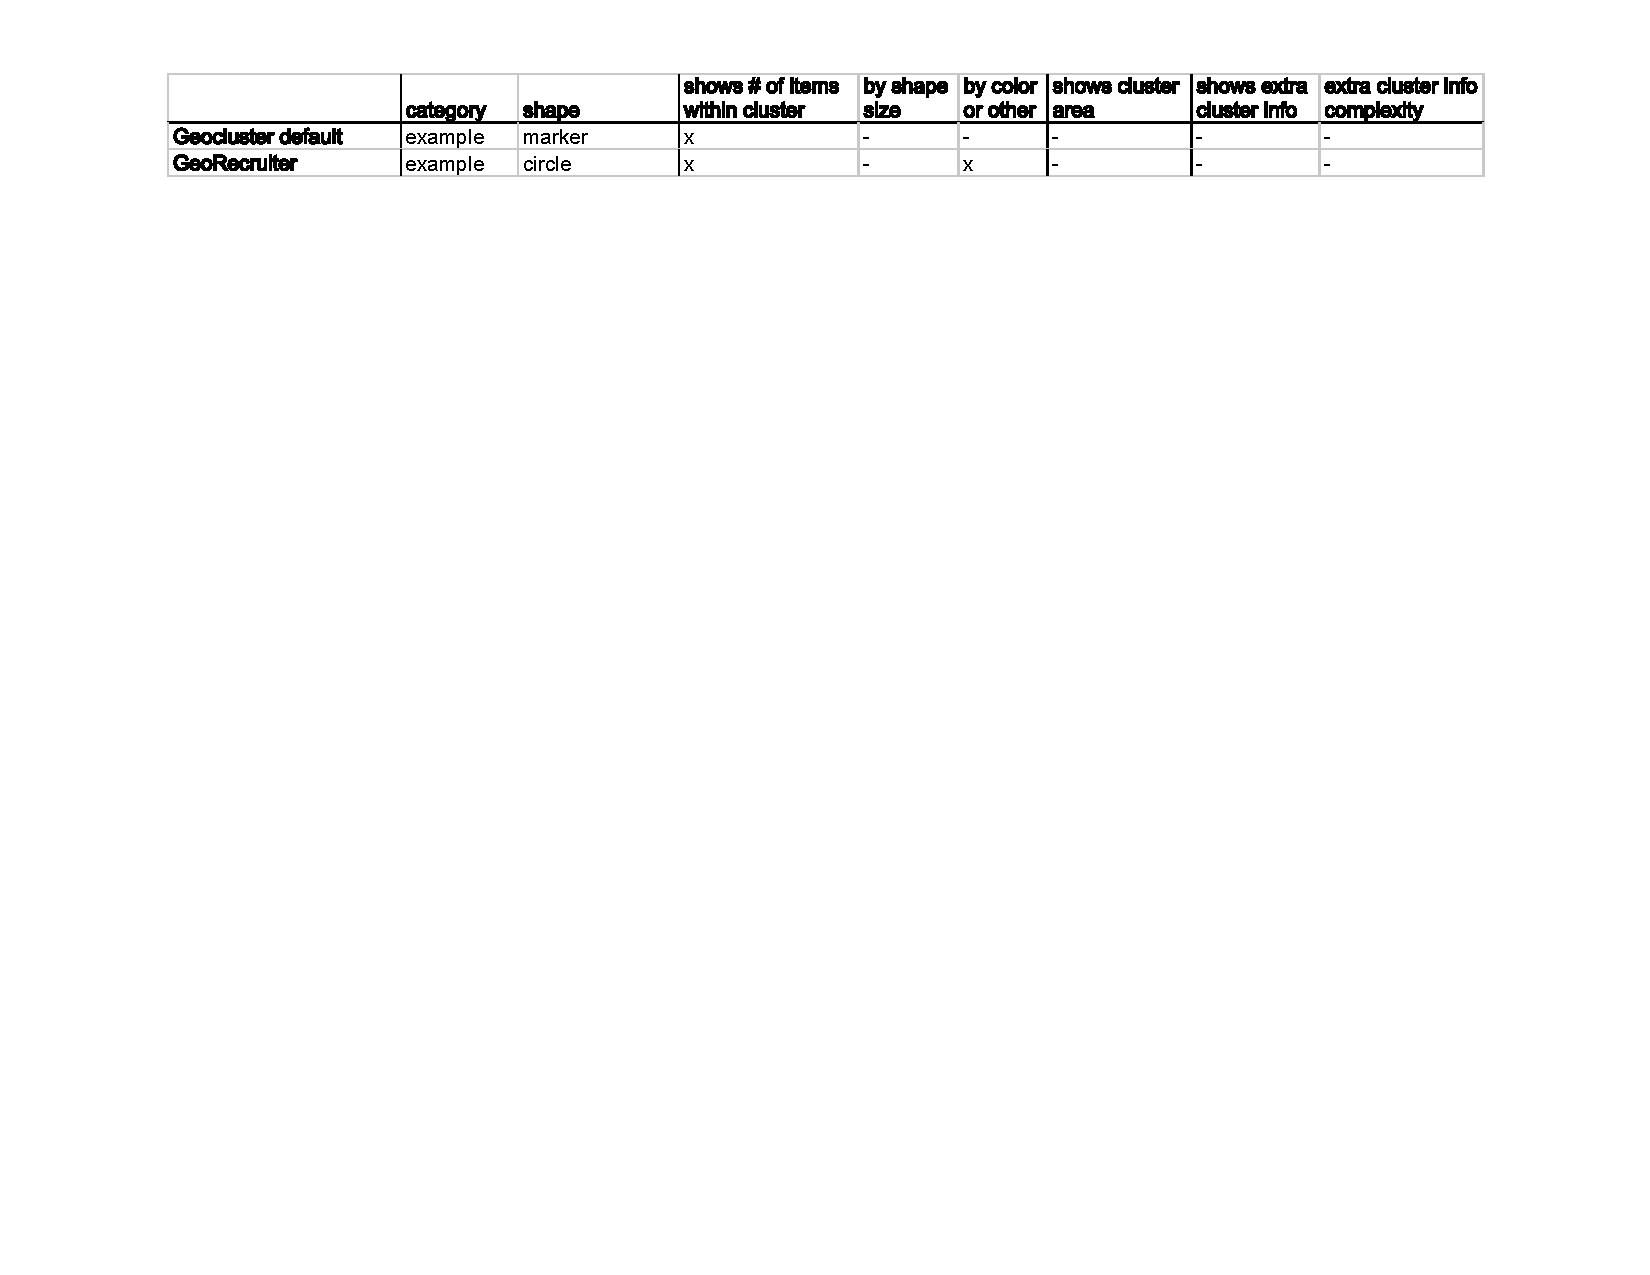
\includegraphics[width=1.2\textwidth]{figures/vis_eval_geocluster.pdf}
    \caption{Evaluation of Geocluster visualization techniques for clusters on a map. Legend:~`x':~yes,~`\textasciitilde': possibly, `-': no.}
    \label{fig:vis-eval-geocluster}
  \end{center}
\end{figure}

Next, the evaluation of visualization techniques for clusters on map presented in \ref{chapter:eval-vis} is applied to the two Geocluster implementations as illustrated in figure \ref{fig:vis-eval-geocluster}. It reiterates some key aspects identified by the previous discussion of clutter reduction criteria.

\textbf{Cluster sizes}: Both visualizations show the number of items within a cluster, but only the GeoRecruiter example uses color and none of them encodes the size of a cluster into the shape size. As naturally, a cluster with more items can be visualized larger than smaller clusters, the algorithm could be improved for growing clusters by their size. The bigger size of a cluster would therefore reduce the distance to its neighbor clusters, potentially merging additional neighbors into it. Andrew Betts describes a similar approach under the term \textit{``Grid based viral growth argorithm''}~\cite{web:clustering-google}.

For low zoom levels, the roundtrip to the server for fetching a separate clustered result on every bounding box change can be an overhead. Christopher Calid\footnote{\url{http://drupal.org/user/210499}} proposes a way of ``Progressively enhance server-side with client-side clustering''\footnote{\url{http://drupal.org/node/1914704}}. The intention is to switch from server-side clustering at higher zoom levels to client-side clustering for lower zoom levels.


\section{Further evaluation}

The third objective on integration and extensibility defined in chapter \ref{chapter:objective-integration} has been fulfilled by the Geocluster module as it integrates with Views, Views GeoJSON and other Drupal mapping modules. In addition, the implementation of the clustering algorithm can be extended using plugins as explained in chapter \ref{chapter:impl-alg}. Geocluster was also released under the GPL license as required by objective \ref{chapter:open-source}. With regards to objective \ref{chapter:objective-use-cases}, a demo use case has been implemented that show cases all the functionality needed. Also, the GeoRecruiter use case has been prototyped.
 
While most objectives have been reached, there are still many parts of the Geocluster implementation that can be improved upon. For example, the way that the Drupal mapping stack integrates with the Views module isn't designed for processing clustered results. The current implementation of Geocluster performs various workarounds in order to inject clustered results into the process. Especially for the Solr-based implementation this leads to code-duplication because in the standard case results are processed as arrays while in the other case, results need to be PHP objects. If possible, a cleaner way of integrating clustering with the related modules is desirable.   


\section{Conclusions}

Writing this thesis and implementing Geocluster was basically a process of over one year. Before starting the thesis, I conducted a research project named AustroFeedr\footnote{\url{http://www.austrofeedr.at/}} on real-time processing technologies for aggregating, processing and visualizing data with Drupal. One main aspect of AustroFeedr was a Drupal-based visualization component using OpenLayers maps. After I had completed AustroFeedr by the end of 2011, I researched Drupal and mapping related topics for writing this master thesis in Software Engineering \& Internet Computing at Technical University Vienna.

The topic server-side clustering for Drupal was decided upon thanks to recommendation by Th\'eodore Biadala\footnote{\url{http://drupal.org/user/598310}}, an active JavaScript and maps contributor in the Drupal community who I met at the Frontend United conference in Amsterdam, April 20-22. After doing some initial research and prototyping, I organized a mapping sprint at Drupal Developer Days Barclona\footnote{\url{http://groups.drupal.org/node/234168}}. This is where Nick Veenhof\footnote{\url{http://drupal.org/user/122682}}, active Apache Solr contributor within the Drupal community, came up with the idea of researching Geohash for realizing an efficient clustering algorithm.

It took until September 2012, when I implemented a first prototype of the PHP-based clustering algorithm and figured out basic integration needs for to make the clustering task work with Drupal. From then, several iterations and alpha releases of Geocluster led to completing MySQL and Solr-based clustering by the end of 2012. As by finishing this thesis in April 2013, performance tests have been concluded for Geocluster and a first beta release has been published.

There has already been some positive feedback from people interested in using Geocluster as a drop-in solution to create scalable maps using server-side clustering. On the other hand, I have to admit that integrating clustering into a complex stack such as the Drupal mapping stack has its advantages and disadvantages. Geocluster does a decent job at clustering data server-side, but the tight integration into the Drupal stack also comes at the cost of overhead and complex integration code. For a person that has the expertise in writing code, it might make sense to create a custom server-side clustering solution for a specific purpose without depending on a number of separate modules. Still, the generic approach has the benefit of others potentially being able to use the Geocluster module. Writing this thesis was both challenging and fun. Drupal is a steadily growing team of contributors of Free and Open Source software. Being able to share my works with such a great community has been a rewarding experience and a solid source of motivation. 

\section{Future work}

Direct community feedback and indirect indicators like the project usage statistics will show if and how the Geocluster module is used by others. As stated before, there are many implementation details that can be enhanced. At epiqo, we are planning to incorporate Geocluster for location-based searches of large-scale job portals based on the Recruiter distribution as stated in chapter \ref{chapter:use-case-georecruiter}. 
